\documentclass[10pt]{article}


\usepackage[utf8]{inputenc}
\usepackage[T1]{fontenc}
\usepackage[frenchb]{babel}

\usepackage{algorithm}
\usepackage{algorithmic}
\usepackage[T1]{fontenc}
\usepackage{enumitem}
\usepackage{hyperref}
\usepackage{graphicx}
\usepackage{color}
\usepackage{listings}
\usepackage{wrapfig}
\usepackage{amsfonts}
\usepackage{amsmath}
\usepackage{mathtools}
\usepackage[hmargin=1.25in,vmargin=1.25in]{geometry}
\usepackage{framed}
\usepackage{mathenv}
\usepackage{blkarray}

%title setuplisting
\title{Projet WEB de groupe}
\author{
  Gangyue CHEN \\
  Louis LAFUMA \\
  Baptiste LAMBERT \\
  Romain PEREIRA
}
\date{22/05/2018}

% table of contents setup
\renewcommand{\contentsname}{Sommaire}
\usepackage{etoolbox}
\patchcmd{\thebibliography}{\section*{\refname}}{}{}{}

\setlength{\parindent}{0cm}
\setlength{\parskip}{1ex plus 0.5ex minus 0.2ex}
\newcommand{\hsp}{\hspace{20pt}}
\newcommand{\HRule}{\rule{\linewidth}{0.5mm}}

\hypersetup{
  colorlinks,
  citecolor=black,
  filecolor=black,
  linkcolor=blue,
  urlcolor=red
}

\begin{document}
  \begin{titlepage}
    \begin{sffamily}
      \begin{center}
	
	\textsc{\LARGE ENSIIE}\\[2cm]
	\textsc{\Large Rapport de projet}\\[1.5cm]
	% Title
	\HRule \\[0.4cm]
	{ \huge \bfseries Projet web en groupe ENSIIE 1A 2018\\[0.4cm] }
	\HRule \\[2cm]
	
	\begin{minipage}{0.4\textwidth}
	  \begin{flushleft} \large
	    Guangyue \textsc{Chen}\\
	    Louis \textsc{Lafuma}\\
	    Baptiste \textsc{Lambert}\\
	    Romain \textsc{Pereira}\\
	  \end{flushleft}
	\end{minipage}
	\begin{minipage}{0.4\textwidth}
	  \begin{flushright} \large
	    \emph{Encadrants :} \\
	    Thomas \textsc{Comes}\\
	    Nassim \textsc{Kirouane}\\
	    Rémi \textsc{Parpaillon}\\
	  \end{flushright}
	\end{minipage}
	\vfill
	% Bottom of the page
	{\large 22/05/2018}
      \end{center}
    \end{sffamily}
  \end{titlepage}
  \maketitle
  \tableofcontents
  
  \section*{Préambule}
  Ce projet est réalisé dans le cadre de nos études à l'ENSIIE.
  Les objectifs sont d'apprendre à concevoir et développer des applications web utilisant un serveur de bases de données,
  et prendre conscience des problématiques d’organisations d’équipes et de répartition des tâches.
  
  \newpage
  \section{La problématique}
    L'idée du projet part d'un constat simple.
    Dans les écoles supérieures, les sports traditionelles (football, basketball, ...)
    sont bien représentés, et organisés dans des ligues universitaires qui sont en place depuis des dizaines d'années.
    
    Cependant, dans le domaine de l'e-sport (compétition de jeux-vidéos), aucunes structures solides n'est en place.
    
    C'est pourquoi, nous avons decidé de travailler à l'élaboration d'un tel plateforme, dont l'objectif à long terme
    et de centraliser toutes les compétitions intra-universitaire sur une seule et même plateforme: ULC ('University League Championship').
    
  
  \newpage
  \section{Solution technique}
    \subsection{Organisation du travail}
      \subsubsection{Organisation général}
	Un 'fork' du dépôt Github a été effectué, puis mis en privé. Guangyue travaille sous MacOSX, les autres sous Linux.
	Nous n'avons pas rencontré de problèmes de compatibilités, seulement de légères difficultés les 1ers jours pour configurer Docker.
	Nous avons developpé sous PHP-Storm, Eclipse et Sublime-text selon les préférences.
      \subsubsection{Répartition des rôles}
	Romain PEREIRA et Guangyue CHEN se sont occupés du Back-end : Romain a construit l'architecture MVC du site (et l'API),
	et Guangyue s'est spécialisé sur l'intégration du jeu PUBG.
	
	Louis LAFUMA et Baptiste LAMBERT ont developpé certaines parties visuelles du site.
    \subsection{Back-end}
      \subsubsection{Base de données}
	La base de données relationelle peut être representée par le diagramme UML suivant.
	\newline
	(La transcription SQL du modèle est disponible dans le fichier 'data/db.sql'):
	\begin{figure}[H]
	  \begin{center}
	    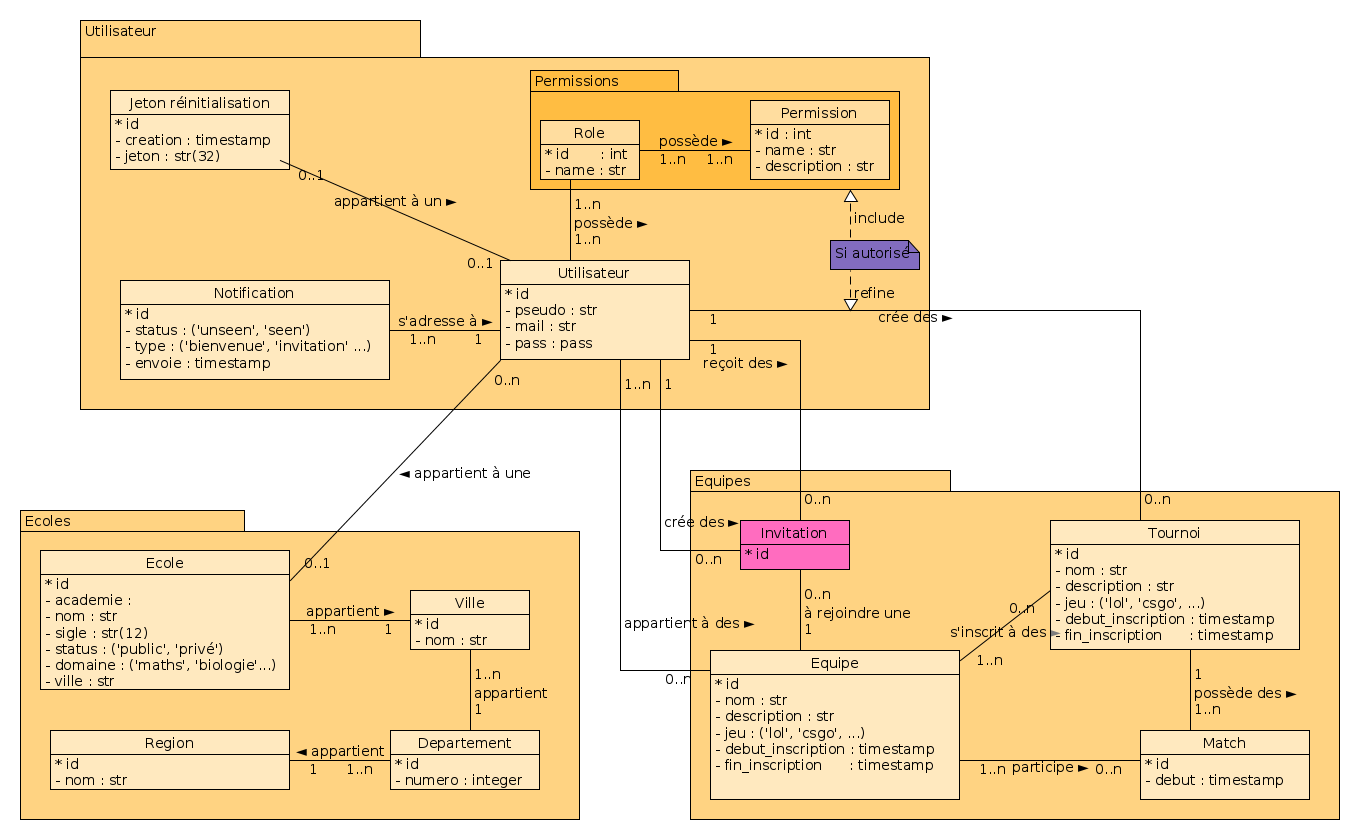
\includegraphics[width=16.0cm,keepaspectratio]{./images/uml.png}
	  \end{center}
	  \caption{\textit{Schéma UML de la base de données}}
	  \label{uml}
	\end{figure}
      
	\paragraph{Permission} Représente une permission ponctuelle (créer une équipe, créer un tournoi, bannir un joueur, inscrire son équipe...)
	\paragraph{Rôle} Représente une ensemble de permissions (administrateur: toutes les permissions, modérateur: bannir un joueur, ...).
	\paragraph{Utilisateur} Possèdent différents rôles, et donc toutes les permissions liées aux rôles.
	Contient les informations relative à un utilisateur enregistré sur le site: mail, pseudo, mot de passe...
	
	Le mot de passe est hashé à l'aide de la fonction PHP 'password\_hash'.
	On protège ainsi efficacement l'accès par un tier au compte de l'utilisateur.
	(les détails techniques ne seront pas présentés ici, voir documentation \ref{password_hash} et \ref{password_salt})
	
	\paragraph{Notification} Un message destiné à attirer l'attention de l'utilisateur du site (e.x: le notifie d'une invitation à rejoindre une équipe)
	\paragraph{Jeton de réinitialisation} Une chaîne de 32 caractères générées aléatoirement.
	Ce jeton est généré et envoyé par mail à un utilisateur s'il a oublié son mot de passe.
	Il a alors 15 minutes pour changer son mot de passe en accédant au service consacré à cet effet.
      
	Une base de données a été généré à partir de la page Wikipédia \ref{ecole_ingé}.
	Les données ont été extraite de la page, au format csv, à l'aide d'un programme Python (et de la bibliothèque BeautifulSoup \ref{beautifulsoup}).
	
	Cette base de donnée aura 2 utilités principales : auto-complétion pour la recherche, et organisation de tournois par région.
	Elle permettra également d'avoir des statistiques par région (fait t'on plus d'e-sport à Angers ou bien à Paris).
	
	\paragraph{Equipe} Les joueurs peuvent créer des équipes, inviter d'autres joueurs dans leur équipes, et rejoindre lorsqu'une invitation est reçu.
	\paragraph{Tournoi} Les utilisateurs possèdant les permissions peuvent rejoindre et créer des tournois
	\paragraph{Match} Les utilisateurs ayant la permission peuvent créer des matchs dans un tournoi.
	Ils peuvent également être généré aléatoirement lors de la création d'un tournoi.

      \newpage
      \subsubsection{L'architecture du site}
	Le site suit une architecture MVC classique.
	La distinction entre les dossiers 'public' et 'src' est clair:
	\begin{itemize}[label=-]
	  \item 'public' : contenu auxquelles l'utilisateur à accès par son navigateur. La lecture des sources de ce dossier n'a aucunes conséquences sur la sécurité du site.
	  Il contient l'API 'REST' public, et une page d'index qui fait appele au Controller.
	  \item 'src': contenu 'privé', auxquelles seuls les développeurs ont accès. Il est separé en 3 sous-dossiers (Model/View/Controller).
	  L'architecture a été conçu de sorte à scale efficacement, et à pouvoir travailler à plusieurs en parallèle sur le projet en minimisant les conflits.
	\end{itemize}
	Le code est amplement commenté, et une attention particulière a été porté à sa clarté.
	Ainsi, nous vous invitons à regarder directement les sources pour comprendre l'architecture en profondeur.
	
      \begin{figure}[H]
	\begin{center}
	  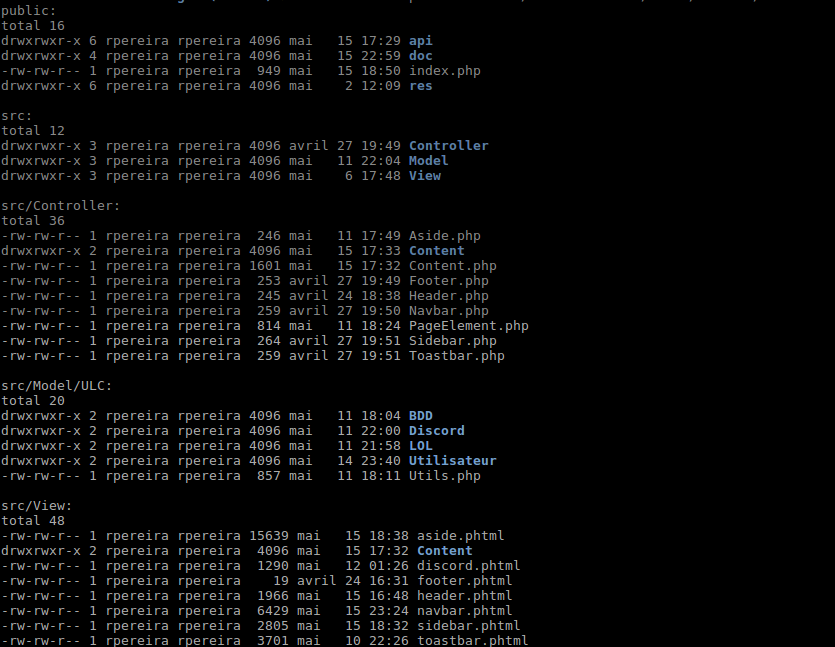
\includegraphics[width=16cm,keepaspectratio]{./images/architecture.png}
	\end{center}
	\caption{\textit{Liste des sources}}
	\label{architecture}
      \end{figure}
      
      \newpage
      \subsubsection{API 'REST'}
	Une API a été implementé sur le modèle REST.
	
	La documentation a été généré via Doxygen, et est accessible à l'adresse \href{http://localhost:8080/doc/html/files.html}{\textit{http://localhost:8080/doc/html/files.html}}.
	
	Cependant, elle ne peut pas être entièrement considéré comme totalement 'REST', car le serveur enregistre des informations dans la session PHP,
	ce qui entre en contradiction avec le principe \ref{api_rest_session}. La satisfaction d'autres principes du 'REST' est également sujet à débat.
	
	Mais elle reste pratique et ouverte: le client du site a été conçu en utilisant très largement cette API. (voir './res/js/api.js')

      \begin{figure}[H]
	\begin{center}
	  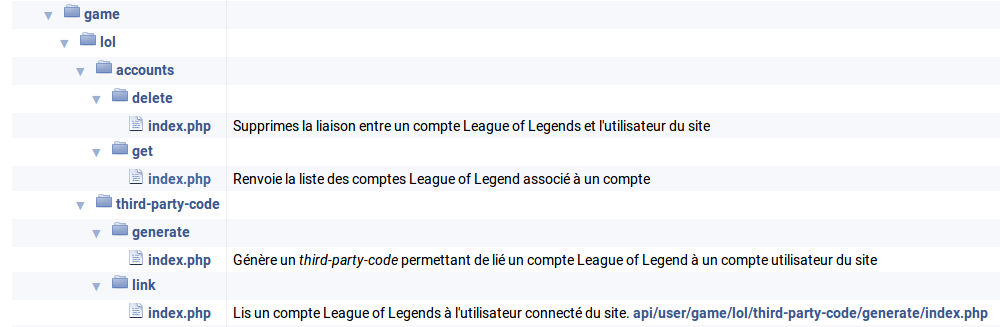
\includegraphics[width=14cm,keepaspectratio]{./images/api.png}
	\end{center}
	\caption{\textit{Partie de la page d'accueil de la documentation}}
	\label{api}
      \end{figure}
      
      \begin{figure}[H]
	\begin{center}
	  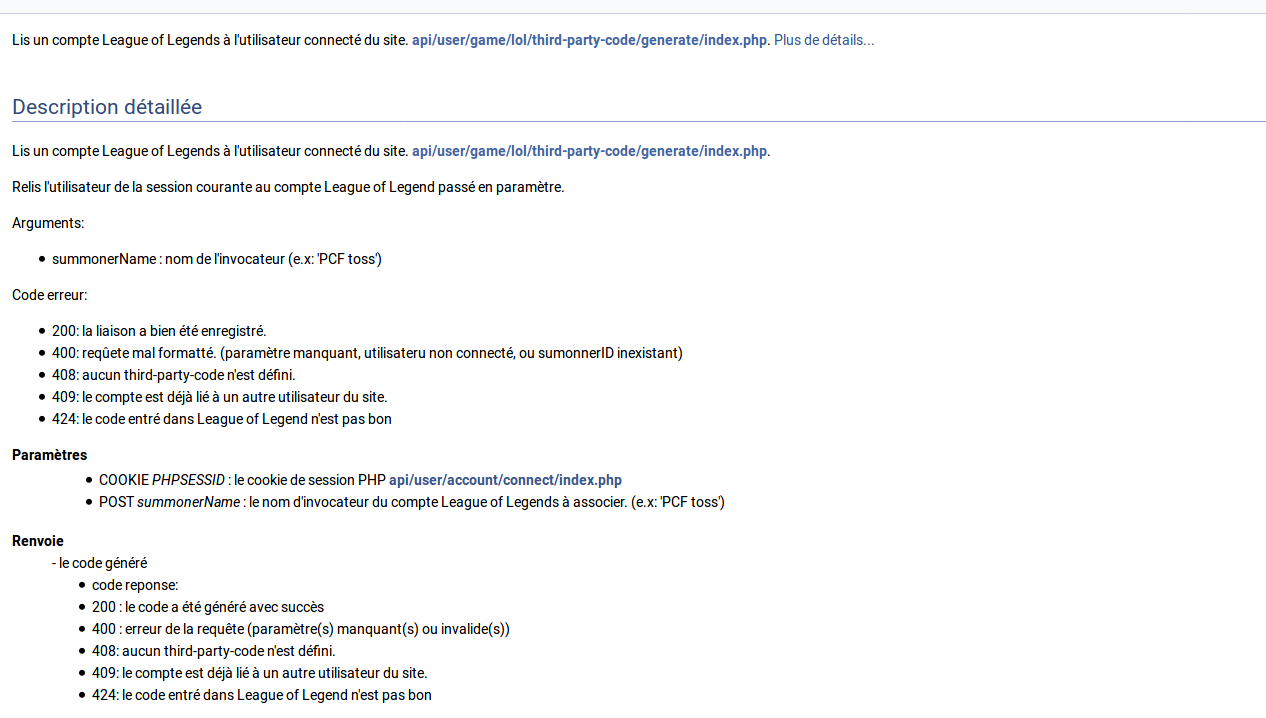
\includegraphics[width=14cm,keepaspectratio]{./images/link_account.png}
	\end{center}
	\caption{\textit{Détail d'une requête (lié un compte Lol à l'utilisateur du site)}}
	\label{link_account}
      \end{figure}
     
      \subsubsection{API externe des jeux}
	Afin d'automatiser le système de tournois, d'effectuer des statistiques, des classements, etc... il faut des données.
	Ces données sont bien souvent garder par les fournisseurs de jeux vidéos.
	Récuperer ces données est donc la clef du projet.
	
	Voici les différents jeux envisagés, et leur politique quant aux partages des données de jeux:
	
	\paragraph{League of Legends - Riot Games}  dispose d'une API public restreinte.
	Afin de pouvoir accéder à toutes les fonctionnalités de l'API (créer des tournois...),
	il faut déposer un projet sur leur site, qui après une étude des developpeurs de Riot, sera accepté ou non.
	Le projet à d'abord été rejeté car il n'était pas assez précis.
	Après avoir ajouté ces précisions, le projet a finalement été accepté et nous avons pu obtenir une clef d'API.
	(cette dernière est privé, nous avons donc joint une clef factice dans les sources du rendu, les fonctionnalités liés à cette API ne fonctionneront donc pas si vous souhaitez tester le site en local)
	
	\paragraph{Fortnite} : Epic Games (la boîte qui gère le jeu) ne fournit pas d'API officiel, et n'ont à priori pas l'intention de le faire...
	
	\paragraph{PUBG} : dispose d'une API complète qui fonctionne similairement à celle de Riot Games.
	
	\paragraph{Hearthstone (Blizzard)} ne dispose pas encore d'une API.
	Cependant, Blizzard dispose d'un portail developpeur (voir \ref{blizzardapi}) proposant des API pour leurs autres jeux (World of Warcraft et Diablo 3).
	Ils ont annoncé l'arrivé d'une API Hearthstone. Tout n'est donc qu'une question de temps pour intégrer le jeu au site.

    \newpage
    \subsection{Front-end}
      \subsubsection{Le 'layout'}
	Le site a été construit en suivant cette leçon de \href{https://www.w3schools.com/css/css_website_layout.asp}{\textit{W3Schools}}.
	
	La barre de navigation (navbar), la barre sur le coté gauche (sidebar), et la barre à droite (asidebar) sont fixes,
	et leur contenu varient selon l'état du client (connecté ou non, rôles...)
	
	Le centre du site contient le contenu de la page, et varient selon la page que l'utilisateur visite.
	
	\begin{figure}[H]
	  \begin{center}
	    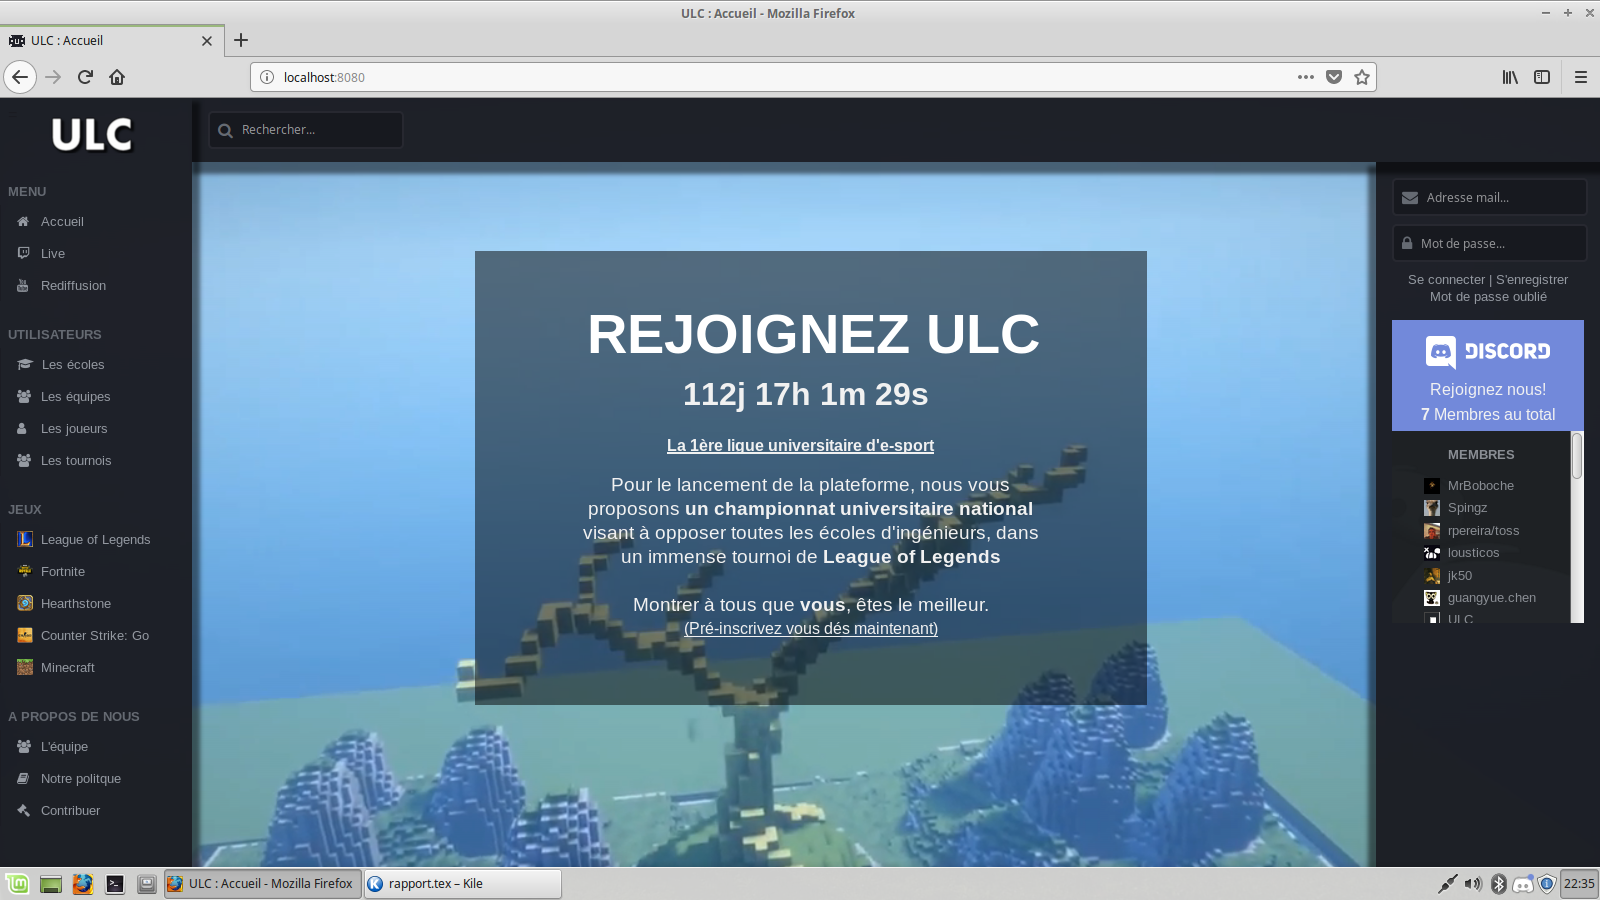
\includegraphics[width=12cm,keepaspectratio]{./images/site.png}
	  \end{center}
	  \caption{\textit{Page d'accueil du site (non connecté)}}
	  \label{site}
	\end{figure}
	
	\begin{figure}[H]
	  \begin{center}
	    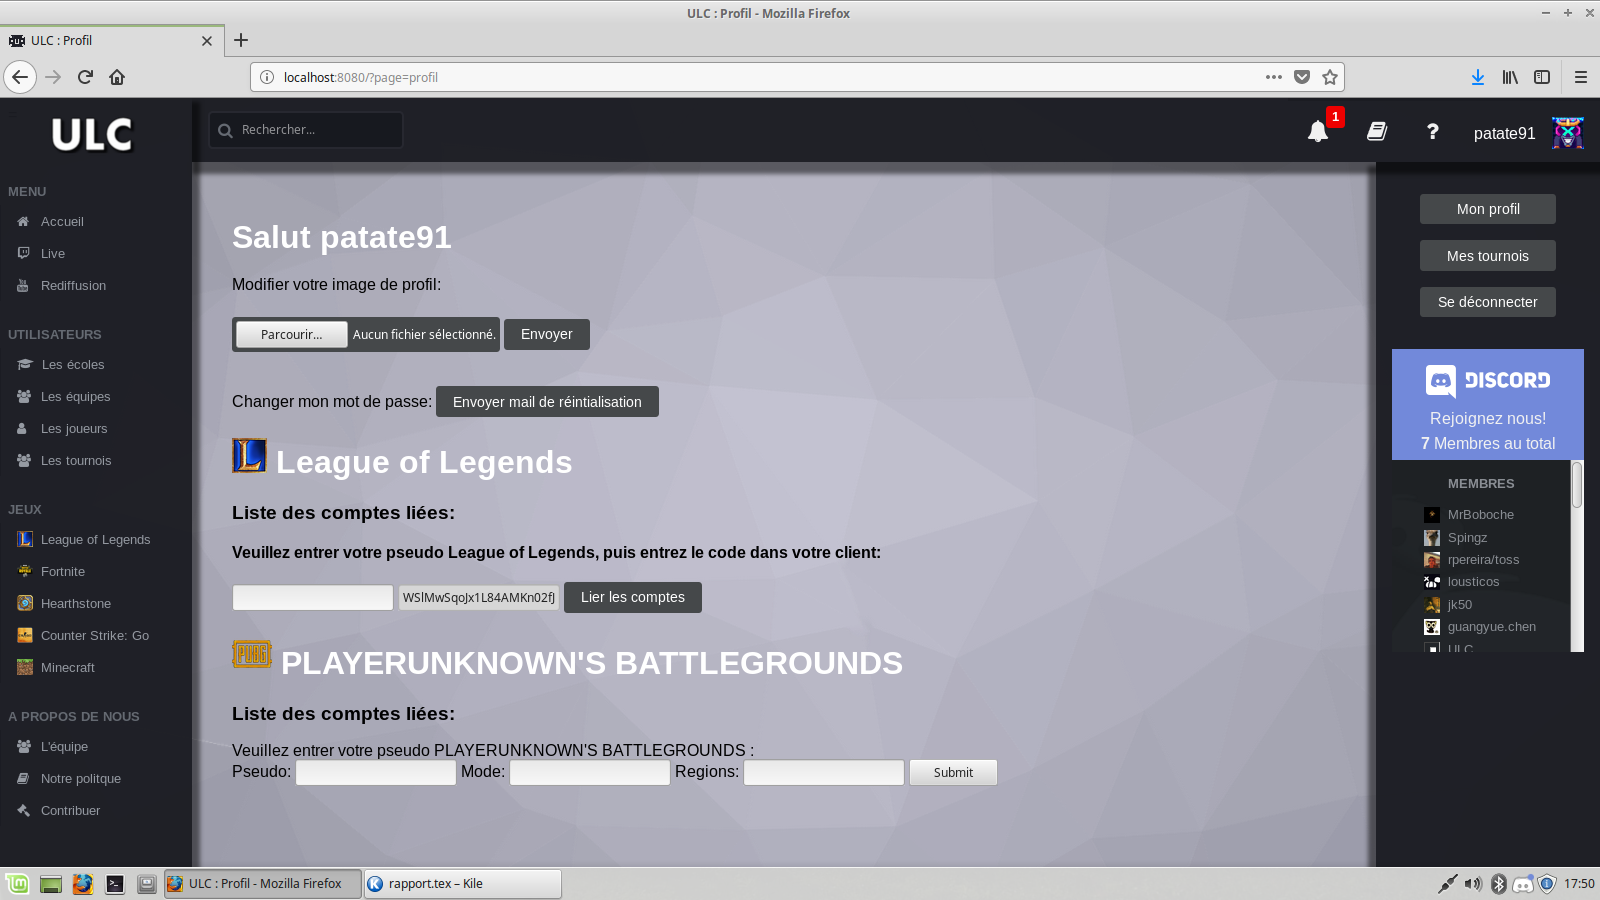
\includegraphics[width=12cm,keepaspectratio]{./images/profil.png}
	  \end{center}
	  \caption{\textit{Page de profil d'un joueur (connecté)}}
	  \label{profil}
	\end{figure}
      
      \subsubsection{Discord}
	Le widget dans la 'asidebar' a été programmé à l'aide de l'API Discord (\ref{discordapi}), et d'un wrapper PHP (voir 'discord.phtml').
	Cette API se configure simplement: chaque administrateur du Discord à accès à une clef d'API sans restrictions.
	
      \subsubsection{Notification}
	Le système de notification 'Facebook-like' fonctionne en temps réel.
	Le client recupère ces notifications toutes les 5 secondes (par l'intermédiaire de l'API).
	(voir cloche sur la figure \ref{profil})

  \section{Conclusion}
    Le site est loin d'être complet. Certaines fonctionnalités présentées dans ce rapport n'ont pas pu être implémenté par manque de temps.

    Cependant, l'architecture du site et sa base de données sont solides, et permettront d'implémenter les fonctionnalités manquantes rapidement.
    \newline
    \newline
    De plus, il y a eu un vif écho au sein de notre entourage: il y a un certain engouement pour le projet.
    Ainsi, une fois le projet validé pédagogiquement, nous comptons terminer et lancer la plateforme.
    (à l'aide d'amis semi-professionel externe à l'école nottament).
    \newline
    \newline
    En s'inspirant des débuts des différentes fédérations sportives (Fédération Française de Football),
    nous souhaiterions déclarer une association loi de 1901, et offrir aux joueurs des tournois avec prix.
        \newline
    \newline
    Plusieurs modèles économiques ont été envisagés (participation au tournoi gratuite ou payante? publicité? diffusion direct sur Twitch? revente des droits à l'image sur les matchs? ...)
    \newline
    \newline
    Nous attendrons cependant d'avoir une équipe complète et soudé pour débattre de cela efficacement.
  
  \newpage
  \section{Références}
  \begin{thebibliography}{}
    
    \bibitem{phpgoodpratices}\label{phpgoodpratices}
    'PHP The Right Way' - \href{https://github.com/codeguy/php-the-right-way/graphs/contributors}{\textit{+200 authors}} \newline
    \href{http://www.phptherightway.com/}{\textit{http://www.phptherightway.com/}}
    \newline
    \newline
    \bibitem{riotapi}\label{riotapi}
    API officiel de Riot Games \newline
    \href{https://developer.riotgames.com/}{\textit{https://developer.riotgames.com/}}
    \newline
    \newline
    \bibitem{discordapi}\label{discordapi}
    API officiel de Discord \newline
    \href{https://discordapp.com/developers/docs/intro}{\textit{https://discordapp.com/developers/docs/intro}}
    \newline
    \newline
    \bibitem{blizzardapi}\label{blizzardapi}
    API officiel de Blizzard \newline
    \href{https://dev.battle.net/io-docs}{\textit{https://dev.battle.net/io-docs}}
    \newline
    \newline
    \bibitem{password_hash}\label{password_hash}
    php.net - password\_hash documentation \newline
    \href{http://php.net/manual/fr/function.password-hash.php}{\textit{http://php.net/manual/fr/function.password-hash.php}}
    \newline
    \newline
    \bibitem{password_salt}\label{password_salt}
    Salage de mot de passe \newline
    \href{https://en.wikipedia.org/wiki/Salt_(cryptography)}{\textit{https://en.wikipedia.org/wiki/Salt\_(cryptography)}}
    \newline
    \newline
    \bibitem{ecole_ingé}\label{ecole_ingé}
    Liste écoles d'ingénieur en France - Wikipédia \newline
    \href{https://fr.wikipedia.org/wiki/Liste_des_écoles_d'ingénieurs_en_France#Liste_des_207_écoles_françaises_accréditées_au_1er_septembre_2017}{\textit{https://fr.wikipedia.org/wiki/Liste\_des\_écoles\_d'ingénieurs\_en\_France}}
    \newline
    \newline
    \bibitem{beautifulsoup}\label{beautifulsoup}
    BeautifulSoup - Documentation\newline
    \href{https://www.crummy.com/software/BeautifulSoup/bs4/doc/}{\textit{https://www.crummy.com/software/BeautifulSoup/bs4/doc/}}
    \newline
    \newline
    \bibitem{api_rest_session}\label{api_rest_session}
    API REST - Wikipédia \newline
    \href{https://fr.wikipedia.org/wiki/Representational_state_transfer#Sans_état}{\textit{https://fr.wikipedia.org/wiki/Representational\_state\_transfer\#Sans\_état}}
    
  \end{thebibliography}
  
\end{document}
